\subsection{Etherless-server}
\subsubsection{Struttura}
Il compito del modulo etherless-server è ascoltare eventi Ethereum emessi dal modulo etherless-smart e processare questi ultimi, andando ad eseguire operazioni prestabilite. Per realizzare queste funzionalità, abbiamo sviluppato le seguenti classi:
\begin{itemize}
	\item \textbf{SmartManager}: classe astratta le cui derivate consentono l'ascolto di eventi esterni e la generazione di corrispondenti eventi interni. Questa classe consente inoltre la comunicazione di risposte ad etherless-smart tramite il metodo \texttt{sendResponse(...)};
	\item \textbf{ETHSmartManager}: classe derivata da SmartManager, dedicata all'ascolto di eventi Ethereum. Tale ascolto inizia al momento della creazione di un oggetto di questa classe;
	\item \textbf{EventDispatcher}: classe che consente l'emissione di eventi interni, che vengono poi processati dalle opportune classi. All'interno di ogni oggetto di tipo SmartManager, sono presenti tanti oggetti di tipo EventDispatcher quante sono le tipologie di eventi che quest'ultimo è in grado di ascoltare;
	\item \textbf{IEventProcessor}: interfaccia che fornisce metodi utili a processare diversi tipologie di evento;
	\item \textbf{EventProcessor}: classe che implementa l'interfaccia IEventProcessor e definisce metodi per processare ogni tipo di evento ricevuto da uno SmartManager. Contiene riferimenti a tutte le classi necessarie a processare tali eventi, il che fornisce quindi ad EventProcessor il controllo completo del processo di gestione delle richieste;
	\item \textbf{EventData}: classe astratta, le cui classi derivate incapsulano il contenuto dell'evento che è stato ricevuto e che si intende processare;
	\item \textbf{AWSManager}: classe adibita alla gestione della comunicazione con i servizi AWS, in particolare AWS Lambda. Contiene metodi utili all'interazione con la piattaforma, per ogni tipo di richiesta da gestire;
	\item \textbf{AWSDeployer}: funzione Lambda, che consente di effettuare il deployment di funzioni Lambda. Utilizzata, nello specifico, per la costruzione di Lambda deployment packages e per il loro deployment sulla piattaforma;
	\item \textbf{IPFSManager}: classe adibita alla gestione della comunicazione con il servizio IPFS. Fornisce funzionalità utili a gestire file (in formato stringa) trasferiti tramite questo servizio;
	\item \textbf{ConfigUtilities}: classe adibita alla creazione di oggetti di configurazione;
	\item \textbf{ETHSmartConfig}: classe contenente le informazioni di configurazione necessarie ad un oggetto ETHSmartManager per creare un'istanza di contratto Ethereum;
	\item \textbf{AWSConfig}: classe contenente le informazioni di configurazione necessarie ad un oggetto AWSManager per creare un'istanza di servizio Lambda.
\end{itemize}
\subsubsection{Design}
L'architettura del modulo etherless-server è stata progettata in conformità ai principi SOLID, e mantenendo come obiettivi fondamentali la scalabità e l'estensibilità:
\begin{itemize}
	\item \textbf{scalabilità}: facendo riferimento alla caratteristica serverless richiesta dal Proponente per l'architettura del sistema, la porzione preponderante dell'elaborazione viene eseguita dal servizio AWS Lambda. Quest'ultimo è in grado di gestire le richieste e ricalibrare le risorse per ottenere la miglior ottimizzazione possibile, entro un limite di 1000 esecuzioni concorrenti;
	\item \textbf{estensibilità}: per garantire la possibilità di integrare nuove funzionalità all'interno del sistema, senza apportare modifiche sostanziali alla sua struttura, sono state implementate varie scelte progettuali quali:
	\begin{itemize}
		\item l'utilizzo di una lista di callback per l'esecuzione di operazioni in risposta all'ascolto di una particolare tipologia di evento, che consente di introdurre nuove operazioni e classi interessate a processare gli eventi, senza apportare modifiche a codice esistente;
		\item lo sviluppo di SmartManager come classe astratta, che consente di gestire nuove fonti di eventi tramite l'introduzione di una nuova classe derivata da quest'ultima;
		\item lo sviluppo di IEventProcessor come interfaccia, che consente di introdurre nuove implementazioni e modalità di gestione delle richieste;
		\item lo sviluppo di EventProcessor come classe che consente di orchestrare i vari passi di elaborazione di una richiesta. Questo garantisce sempre la possibilità di introdurre interazioni con nuove classi nel processo;
		\item l'utilizzo di ConfigUtilities per la creazione di oggetti di configurazione, garantendo sempre la possibilità di fornire le opportune configurazioni ai nuovi servizi introdotti;
		\item lo sviluppo di EventData come classe astratta, per gestire il contenuto di eventuali nuove tipologie di evento.	
	\end{itemize}
\end{itemize}
Durante la progettazione abbiamo fatto riferimento principalmente a due design pattern:
\begin{itemize}
	\item \textbf{Facade}: come design pattern strutturale per lo sviluppo della classe EventProcessor, che si occupa di orchestrare le chiamate alle opportune classi, per il processing delle richieste ricevute da SmartManager;
	\item \textbf{Dependency injection}: come design pattern architetturale per lo sviluppo delle classi SmartManager, EventDispatcher ed EventProcessor: 
	\begin{itemize}
		\item al momento dell'istanziazione di un oggetto di tipo SmartManager la lista di callback presente all'interno dei suoi EventDispatcher è vuota, quindi non sono presenti dipendenze verso la classe EventProcessor;
		\item la costruzione di un oggetto di tipo EventProcessor, a cui viene fornito un oggetto di tipo SmartManager come parametro (\textbf{Constructor injection}), provoca l'inserimento di un riferimento alle proprie funzioni di elaborazione nelle rispettive liste di callback in SmartManager (\textbf{Setter injection}).
	\end{itemize}
	Quest'operazione ci consente quindi di introdurre una dipendenza da EventDispatcher verso EventProcessor, senza incorrere negli effetti collaterali tipici di una dipendenza circolare.
\end{itemize}
\newgeometry{a4paper,left=1in,right=1in,top=1in,bottom=1in,nohead}
\begin{landscape}
\subsubsection{Diagramma dei package}
	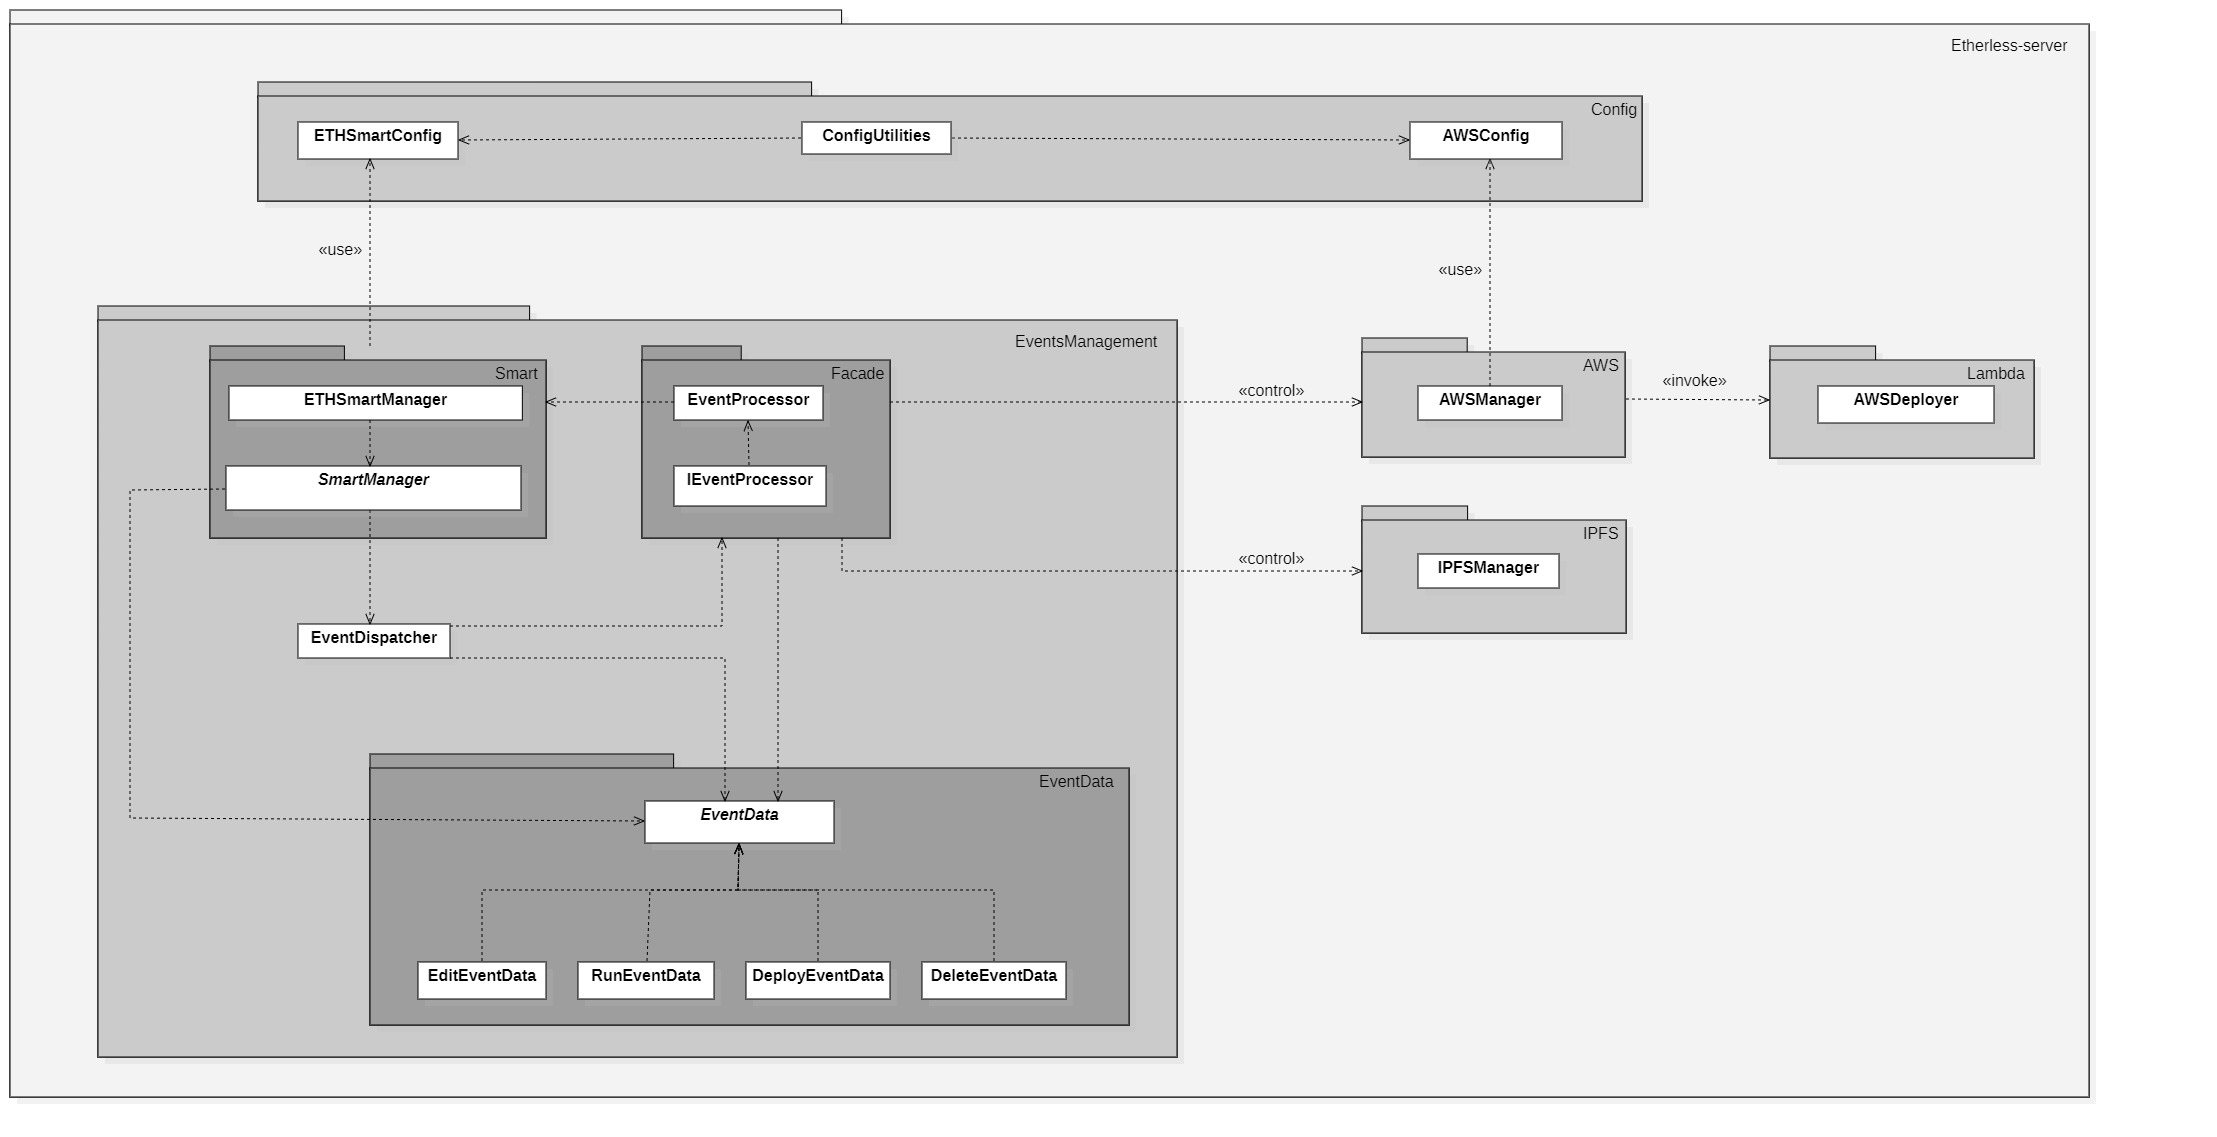
\includegraphics[width=24cm, height=14cm]{././diagrammi/etherless-server/Etherless-server-package.png}
\end{landscape}
\restoregeometry
\newgeometry{a4paper,left=1in,right=1in,top=1in,bottom=1in,nohead}
\begin{landscape}
\subsubsection{Diagramma delle classi}
	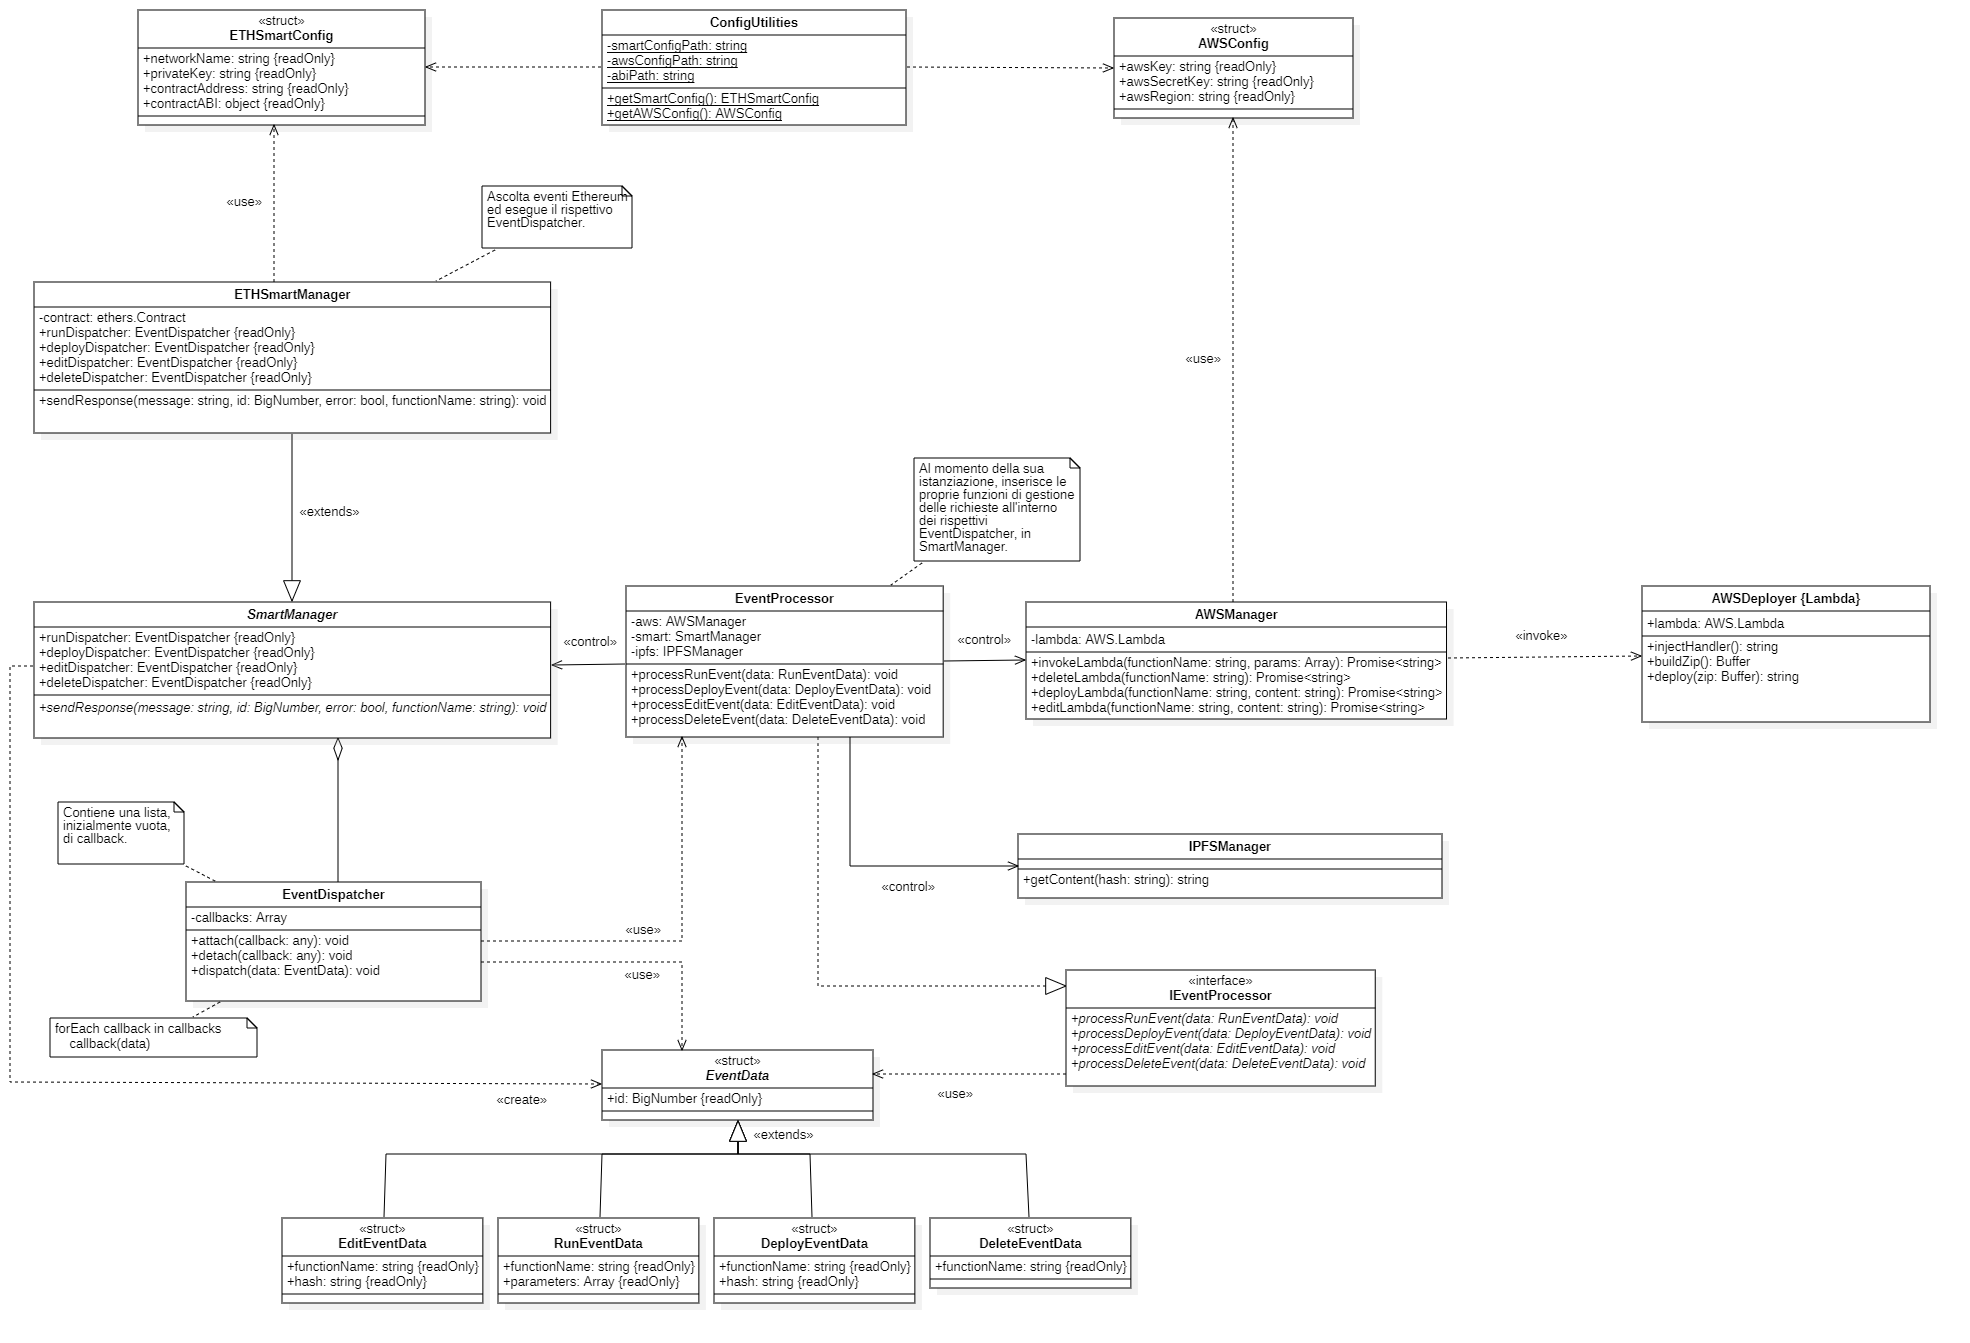
\includegraphics[width=23cm, height=14cm]{././diagrammi/etherless-server/Etherless-server-classi.png}
\end{landscape}
\restoregeometry
\subsubsection{Diagrammi di sequenza}
\begin{figure}[!h]
	\noindent
	\makebox[\textwidth]{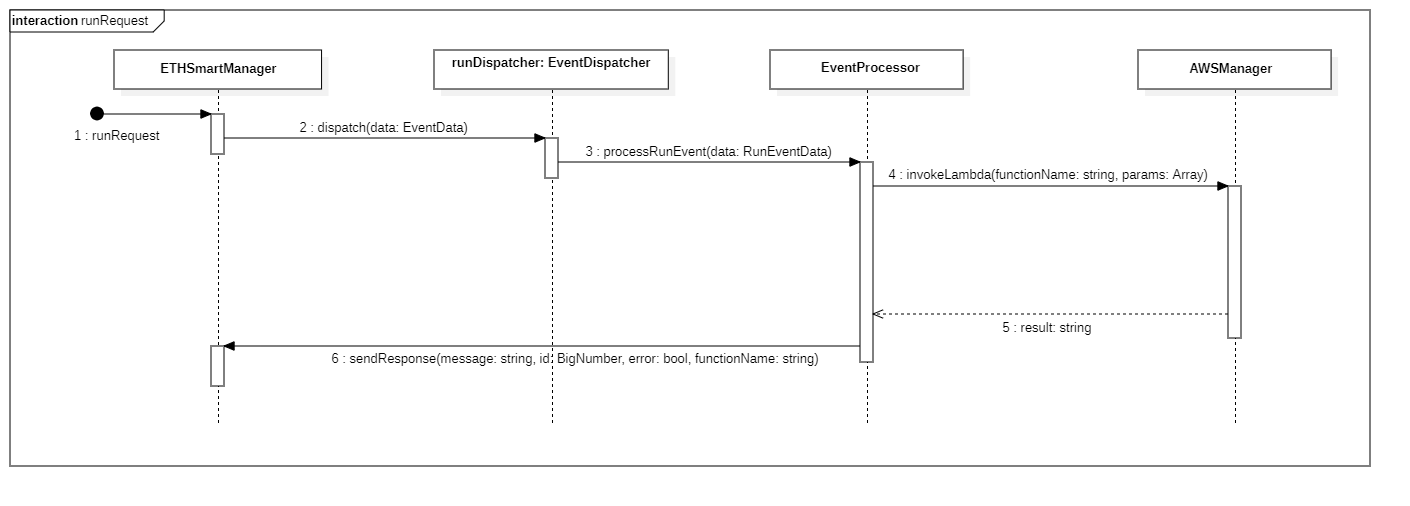
\includegraphics[scale=0.45]{././diagrammi/etherless-server/RunRequest.png}}
	\caption{Diagramma di sequenza dell'esecuzione di una funzione Lambda}
\end{figure}
\begin{figure}[!h]
	\noindent
	\makebox[\textwidth]{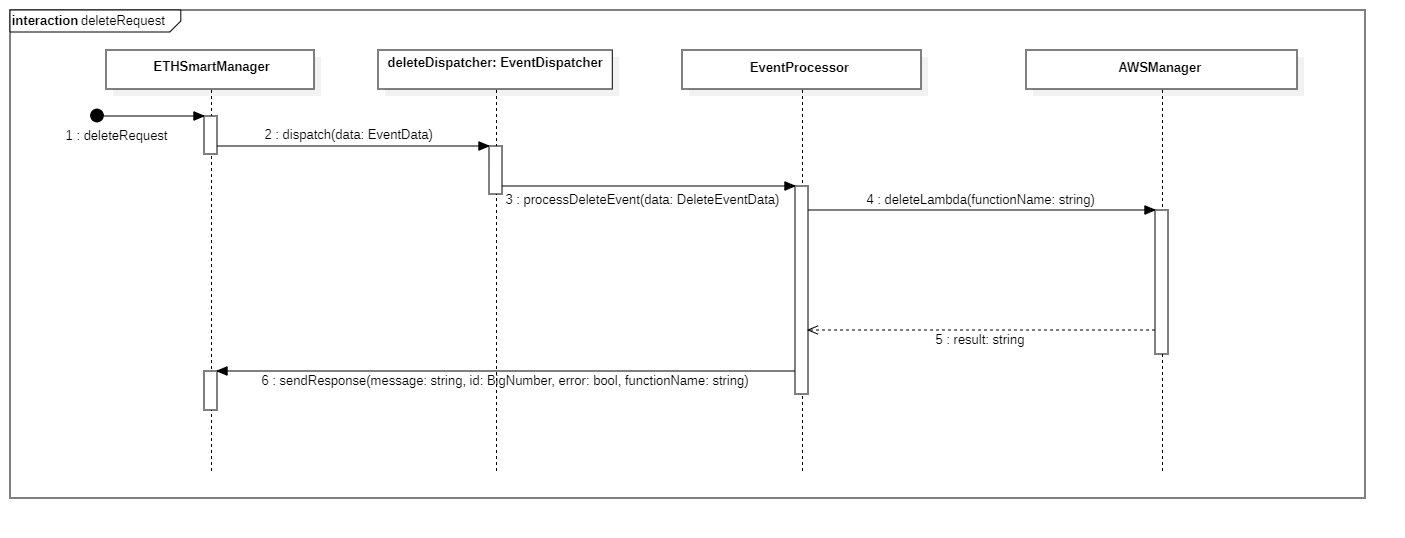
\includegraphics[scale=0.45]{././diagrammi/etherless-server/DeleteRequest.png}}
	\caption{Diagramma di sequenza dell'eliminazione di una funzione Lambda}
\end{figure}
\begin{figure}[!h]
	\noindent
	\makebox[\textwidth]{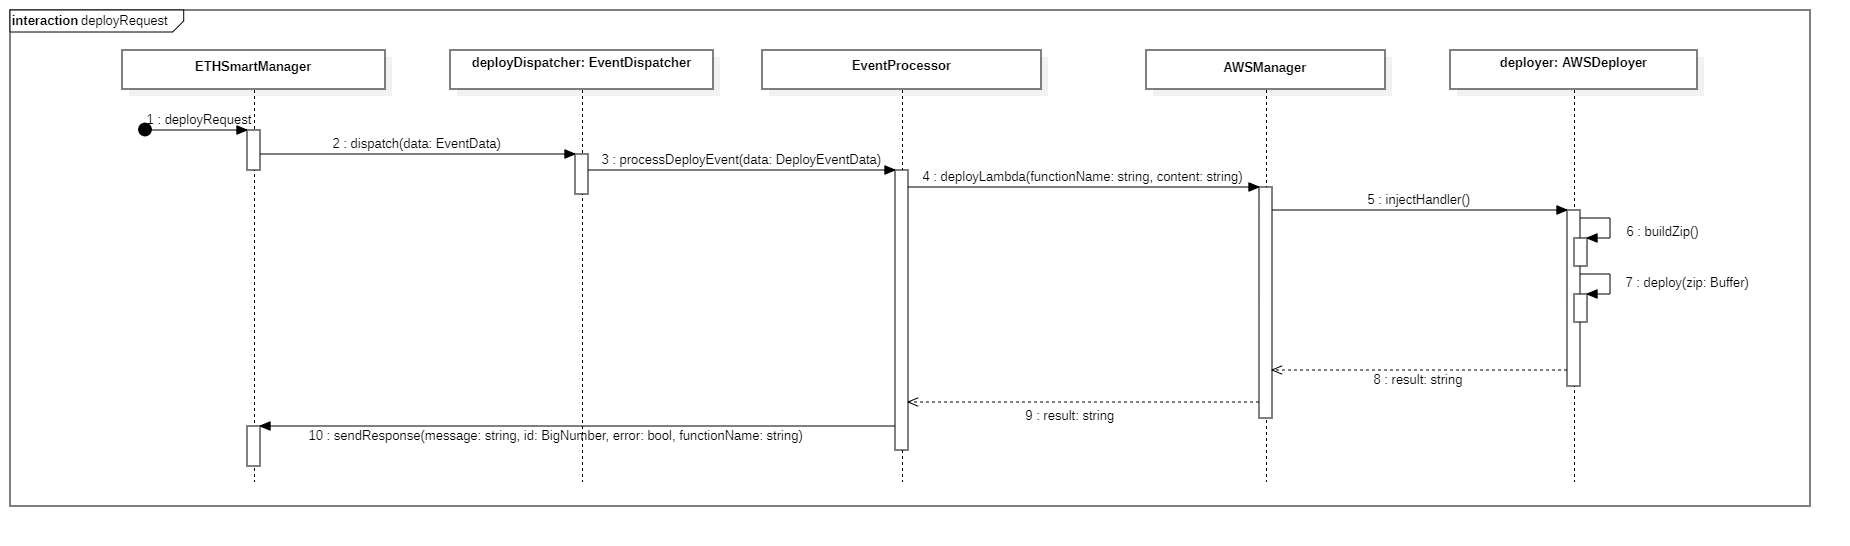
\includegraphics[scale=0.4]{././diagrammi/etherless-server/DeployRequest.png}}
	\caption{Diagramma di sequenza del deployment di una funzione Lambda}
\end{figure}
\begin{figure}[!h]
	\noindent
	\makebox[\textwidth]{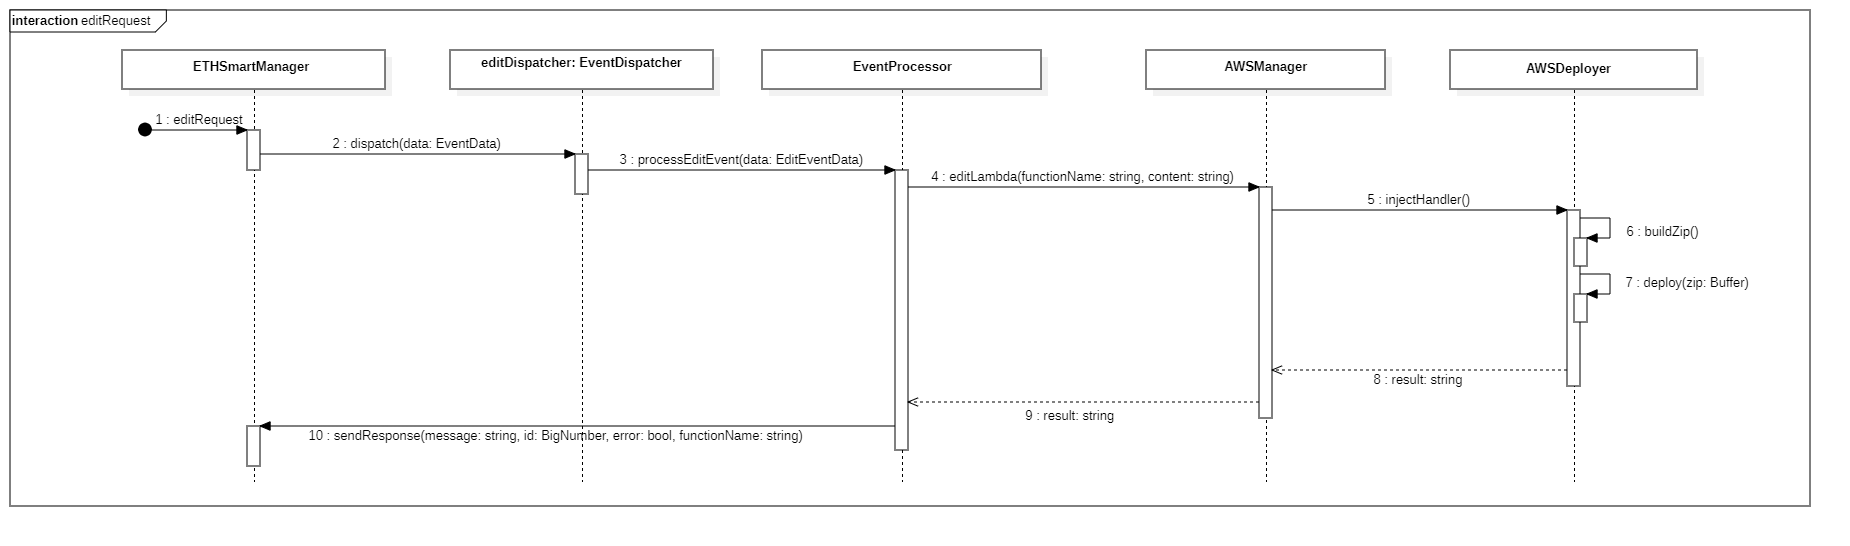
\includegraphics[scale=0.4]{././diagrammi/etherless-server/EditRequest.png}}
	\caption{Diagramma di sequenza della modifica di una funzione Lambda}
\end{figure}


